\begin{titlingpage}

\newcommand\nbvspace[1][3]{\vspace*{\stretch{#1}}}
% allow some slack to avoid under/overfull boxes
\newcommand\nbstretchyspace{\spaceskip0.5em plus 0.25em minus 0.25em}
% To improve spacing on titlepages
\newcommand{\nbtitlestretch}{\spaceskip0.6em}
\pagestyle{empty}

\begin{center}
\bfseries
\nbvspace[1]

\Large Xin Yan\\
\Large Xiao Gang Su\\
\Huge
{\nbtitlestretch\Huge Análisis de regresión lineal}\\
\nbvspace[1]

RESOLUCIÓN DE PROBLEMAS\\
Y APUNTES\\

\nbvspace[1]
\small POR\\
\Large FODE\\[0.5em]
\footnotesize CHRISTIAN LIMBERT PAREDES AGUILERA\\

\nbvspace[2]

\begin{center}
    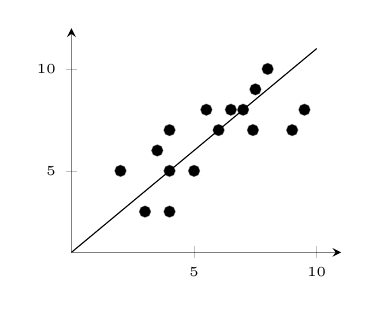
\begin{tikzpicture}
	\begin{axis}[scale=.5,draw opacity =.5,samples=100,smooth, 
	  axis x line=center, 
	  axis y line=center,
	  xlabel style={below right},
	  ylabel style={above left},
	  label style={font=\tiny},
	  tick label style={font=\tiny},
	  enlargelimits=upper] 
	  \addplot[black,opacity=1,domain=0:10]{x+1};
	  \addplot[only marks]table{
	    5  5   
	    4  7
	    3  3
	    4  3
	    4  5
	    3.5 6 
	    2  5
	    7 	8
	    7.4 7
	    5.5 8
	    6  7
	    6.5 8
	    7.5 9
	    8  10
	    9 7
	    9.5 8
	    };
	\end{axis}
    \end{tikzpicture}
\end{center}


\nbvspace[3]
\normalsize

LIBRO EN SU PRIMERA EDICIÓN (Ingles)\\
\large
\nbvspace[1]

\end{center}

\break
\bfseries 

\nbvspace[1]
Título de la obra original:\\
Linear Regression Alalysis \\
Theory and Computing\\
Edición original en lengua inglesa publicada por:\\
World Scientific Publishing Co. Pte. Ltd.\\

\nbvspace[1]

\begin{center}
Sin ninguna revisión de esta obra.\\


\nbvspace[1]
    Propiedad de esta obra:\\ 

    CHRISTIAN LIMBERT PAREDES AGUILERA\\	

    E-mail: soyfode@gmail.com
\end{center}

\nbvspace[1]

Reservados todos los derechos. La reproducción total o parcial de esta obra, por cualquier medio o procedimiento, comprendidos la reprografía y el tratamiento informático, y la distribución de ejemplares de ella mediante alquiler o préstamo públicos, queda rigurosamente prohibida sin la autorización escrita de los titulares del copyright, bajo las sanciones establecidas por las leyes.\\

\center 2020 

\end{titlingpage}


\pagenumbering{roman}

\tableofcontents								%indice

\pagestyle{fancy}
\fancyhead[LE,RO]{\nouppercase{\truncate{0.5\headwidth}{\rightmark}}}
\fancyhead[LO,RE]{\nouppercase{\truncate{0.5\headwidth}{\leftmark}}}


